\documentclass[letterpaper]{article}

%********************************************************
%* latex shortcuts used for libscuff documentation files
%* 
%* homer reid -- 1994--2011
%**************************************************
\usepackage{graphicx}
\usepackage{color}
\usepackage{dsfont}
\usepackage{bbm}
\usepackage{amsmath}
\usepackage{amssymb}
\usepackage{float}
\usepackage{psfrag}
\usepackage{mathdots}
%\usepackage{algorithm}
%\usepackage{algorithmic}
%\usepackage{listings}
\usepackage{array}
\usepackage{url}
\usepackage{arydshln}
\usepackage{fancybox}
\usepackage{fancyvrb}
\usepackage{verbatim}

%--------------------------------------------------
%- boldface greek letters 
%--------------------------------------------------
\newcommand\vbphi{\mathbf{\phi}}
\newcommand\vbPhi{\mathbf{\Phi}}
\newcommand{\vbDelta}{\boldsymbol{\Delta}}
\newcommand{\vbrho}{\boldsymbol{\rho}}
\newcommand{\vbchi}{\boldsymbol{\chi}}

%--------------------------------------------------
%- colors -----------------------------------------
%--------------------------------------------------
\newcommand{\red}[1]{\textcolor{red}{#1}}
\newcommand{\blue}[1]{\textcolor{blue}{#1}}
\newcommand{\green}[1]{\textcolor{green}{#1}}
\newcommand{\atan}{\text{atan}}

%--------------------------------------------------
% general commands
%--------------------------------------------------
\newcommand\Tr{\hbox{Tr }}
\newcommand\sups[1]{^{\hbox{\scriptsize{#1}}}}
\newcommand\supt[1]{^{\hbox{\tiny{#1}}}}
\newcommand\subs[1]{_{\hbox{\scriptsize{#1}}}}
\newcommand\subt[1]{_{\hbox{\tiny{#1}}}}
\newcommand{\nn}{\nonumber \\}
\newcommand{\vb}[1]{\mathbf{#1}}
\newcommand{\numeq}[2]{\begin{equation} #2 \label{#1} \end{equation}}
\newcommand{\pard}[2]{\frac{\partial #1}{\partial #2}}
\newcommand{\pardn}[3]{\frac{\partial^{#1} #2}{\partial #3^{#1}}}
\newcommand{\pf}[2]{\left(\frac{#1}{#2}\right)}
\newcommand{\pp}{{\prime\prime}}
\newcommand{\vbhat}[1]{\vb{\hat #1}}
\newcommand{\mc}[1]{\mathcal{#1}}
\newcommand{\bmc}[1]{\boldsymbol{\mathcal{#1}}}
\newcommand{\mb}[1]{\mathbb{#1}}
\newcommand{\ds}[1]{\displaystyle{#1}}
\newcommand{\primedsum}{\sideset{}{'}{\sum}}
\newcommand{\pan}{\mathcal{P}}

%--------------------------------------------------
%- special libscuff stuff--------------------------
%--------------------------------------------------
\newcommand\ls{{\sc libscuff}}
\newcommand\lss{{\sc libscuff\,}}
\newcommand{\BG}{\boldsymbol{\Gamma}}
\newcommand{\MInt}{\vb{\hat M}}
\newcommand{\NInt}{\vb{\hat N}}
\newcommand{\MExt}{\vb{\check M}}
\newcommand{\NExt}{\vb{\check N}}
\newcommand{\xInt}{\vb{\hat x}}
\newcommand{\xExt}{\vb{\check x}}

%--------------------------------------------------
%-- superscripts for dyadic green's functions 
%--------------------------------------------------
\newcommand{\EEe}{^{\hbox{\tiny{EE}\scriptsize{,$e$}}}}
\newcommand{\MEe}{^{\hbox{\tiny{ME}\scriptsize{,$e$}}}}
\newcommand{\EMe}{^{\hbox{\tiny{EM}\scriptsize{,$e$}}}}
\newcommand{\MMe}{^{\hbox{\tiny{MM}\scriptsize{,$e$}}}}
\newcommand{\EEr}{^{\hbox{\tiny{EE}\scriptsize{,$r$}}}}
\newcommand{\MEr}{^{\hbox{\tiny{ME}\scriptsize{,$r$}}}}
\newcommand{\EMr}{^{\hbox{\tiny{EM}\scriptsize{,$r$}}}}
\newcommand{\MMr}{^{\hbox{\tiny{MM}\scriptsize{,$r$}}}}
\newcommand{\incr}{^{\text{\scriptsize inc},r}}
\newcommand{\incro}{^{\text{\scriptsize inc},r_1}}
\newcommand{\incrt}{^{\text{\scriptsize inc},r_2}}

%%%%%%%%%%%%%%%%%%%%%%%%%%%%%%%%%%%%%%%%%%%%%%%%%%%%%%%%%%%%%%%%%%%%%%
%%%%%%%%%%%%%%%%%%%%%%%%%%%%%%%%%%%%%%%%%%%%%%%%%%%%%%%%%%%%%%%%%%%%%%
%%%%%%%%%%%%%%%%%%%%%%%%%%%%%%%%%%%%%%%%%%%%%%%%%%%%%%%%%%%%%%%%%%%%%%
\newcommand{\MMExt}{\check{\mathcal{M}}}
\newcommand{\MMInt}{\hat{\mathcal{M}}}
\newcommand{\NNExt}{\check{\mathcal{N}}}
\newcommand{\NNInt}{\hat{\mathcal{N}}}
\newcommand{\BMMExt}{\boldsymbol{\check{\mathcal{M}}}}
\newcommand{\BMMInt}{\boldsymbol{\hat{\mathcal{M}}}}
\newcommand{\BNNExt}{\boldsymbol{\check{\mathcal{N}}}}
\newcommand{\BNNInt}{\boldsymbol{\hat{\mathcal{N}}}}
\newpage

%--------------------------------------------------
%- inner products and operator matrix elements  ---
%--------------------------------------------------
\newcommand{\expval}[1]{ \big\langle #1 \big\rangle}
\newcommand{\Expval}[1]{ \Big\langle #1 \Big\rangle}
\newcommand{\inp}[2]{ \big\langle #1 \big| #2 \big\rangle}
\newcommand{\Inp}[2]{ \Big\langle #1 \Big| #2 \Big\rangle}
\newcommand{\INP}[2]{ \bigg\langle #1 \bigg| #2 \Big\rangle}
\newcommand{\vmv}[3]{ \big\langle #1 \big| #2 \big| #3 \big\rangle}
\newcommand{\VMV}[3]{ \Big\langle #1 \Big| #2 \Big| #3 \Big\rangle}

%------------------------------------------------------------
%- shaded box for source code inclusions 
%------------------------------------------------------------
%\definecolor{lightgrey}{rgb}{0.85,0.85,0.85}
%\newcommand{\SourceBox}[1]
% { \begin{mdframed}[backgroundcolor=lightgrey, linewidth=2pt,
%                    tikzsetting={draw=black, line width=2pt,
%                                 dashed, dash pattern= on 5pt off 5pt}] %
%  \begin{verbatim} #1 \end{verbatim} \end{mdframed} \medskip
%}
%\IfFileExists{mdframed.sty}
% { \usepackage{mdframed}
%   \surroundwithmdframed[backgroundcolor=lightgrey, linewidth=2pt,
%                         framemethod=tikz,
%                         skipabove=10pt,
%                         skipbelow=10pt,
%                         tikzsetting={draw=black, line width=2pt,
%                                      dashed, dash pattern= on 5pt off 5pt}
%                        ]{verbatim}
% }
% {
% }
%--------------------------------------------------
%- shaded verbatim for code inclusions
%--------------------------------------------------
\definecolor{lightgrey}{rgb}{0.85,0.85,0.85}
\newenvironment{verbcode}{\VerbatimEnvironment% 
  \noindent
  %{\columnwidth-\leftmargin-\rightmargin-2\fboxsep-2\fboxrule-4pt} 
  \begin{Sbox} 
  \begin{minipage}{\linewidth}
  \begin{Verbatim}
}{% 
  \end{Verbatim}  
   \end{minipage}
  \end{Sbox} 
  \fcolorbox{black}{lightgrey}{\textcolor{black}{\TheSbox}}
} 


\graphicspath{{figures/}}

%------------------------------------------------------------
%------------------------------------------------------------
%- Special commands for this document -----------------------
%------------------------------------------------------------
%------------------------------------------------------------

%------------------------------------------------------------
%------------------------------------------------------------
%- Document header  -----------------------------------------
%------------------------------------------------------------
%------------------------------------------------------------
\title {RF device modeling in {\sc scuff-em}}
\author {Homer Reid}
\date {April 16, 2018}

%------------------------------------------------------------
%------------------------------------------------------------
%- Start of actual document
%------------------------------------------------------------
%------------------------------------------------------------

\begin{document}
\pagestyle{myheadings}
\markright{Homer Reid: The {\sc scuff-em} RF module}
\maketitle

\tableofcontents

%%%%%%%%%%%%%%%%%%%%%%%%%%%%%%%%%%%%%%%%%%%%%%%%%%%%%%%%%%%%%%%%%%%%%%
%%%%%%%%%%%%%%%%%%%%%%%%%%%%%%%%%%%%%%%%%%%%%%%%%%%%%%%%%%%%%%%%%%%%%%
%%%%%%%%%%%%%%%%%%%%%%%%%%%%%%%%%%%%%%%%%%%%%%%%%%%%%%%%%%%%%%%%%%%%%%
\section{Overview}

The {\sc scuff-em} package includes a module for RF device modeling
within the framework of integral-equation electromagnetism.
The core functionality of the module is implemented
within the {\sc scuff-solver} high-level interface to {\sc scuff-em}
and may be accessed either \textbf{(a)} in API form 
from C++ or python programs, or \textbf{(b)} from the command line
via the {\sc scuff-rf} binary application code.

The {\sc scuff-em} RF module extends the existing functionality of the
{\sc scuff-em} core library in two main ways:

\begin{enumerate}
  \item It introduces the notion of a \textit{port.} This is a region
        of your structure (be it an antenna, a coaxial cable, etc.)
        that interfaces with RF circuitry; more specifically, a port
        consists of a positive terminal, into which a current of arbitrary
        complex amplitude is injected,
        and a negative terminal from which the same current is extracted.
        The fields radiated by these currents define the incident field
        in the SIE scattering problem solved by {\sc scuff-em}.

        Ports are defined by geometric entities (points, lines, or
        polygons) identifying regions of meshed structures.
        Information on ports is stored internally in the {\sc scuff-em}
        RF module via data structures named \texttt{RWGPort} and 
        \texttt{RWGPortEdge}.
  \item It introduces a new type of post-processing operation
        to compute the \textit{impedance parameters} of a multiport geometry.
        (All of the varous other types of post-processing calculations offered by
        core {\sc scuff-em}---including computation and visualization of fields,
        induced moments, power, etc.---are available as well.)
\end{enumerate}

In this memo we will discuss the implementation of these features.

%%%%%%%%%%%%%%%%%%%%%%%%%%%%%%%%%%%%%%%%%%%%%%%%%%%%%%%%%%%%%%%%%%%%%%
%%%%%%%%%%%%%%%%%%%%%%%%%%%%%%%%%%%%%%%%%%%%%%%%%%%%%%%%%%%%%%%%%%%%%%
%%%%%%%%%%%%%%%%%%%%%%%%%%%%%%%%%%%%%%%%%%%%%%%%%%%%%%%%%%%%%%%%%%%%%%
\newpage
\section{The concept of an \texttt{RWGPort}}
%####################################################################%
%####################################################################%
%####################################################################%
\begin{figure}
\begin{center}
\begin{tabular}{cc}
\begin{tabular}{c}
\resizebox{0.5\textwidth}{!}{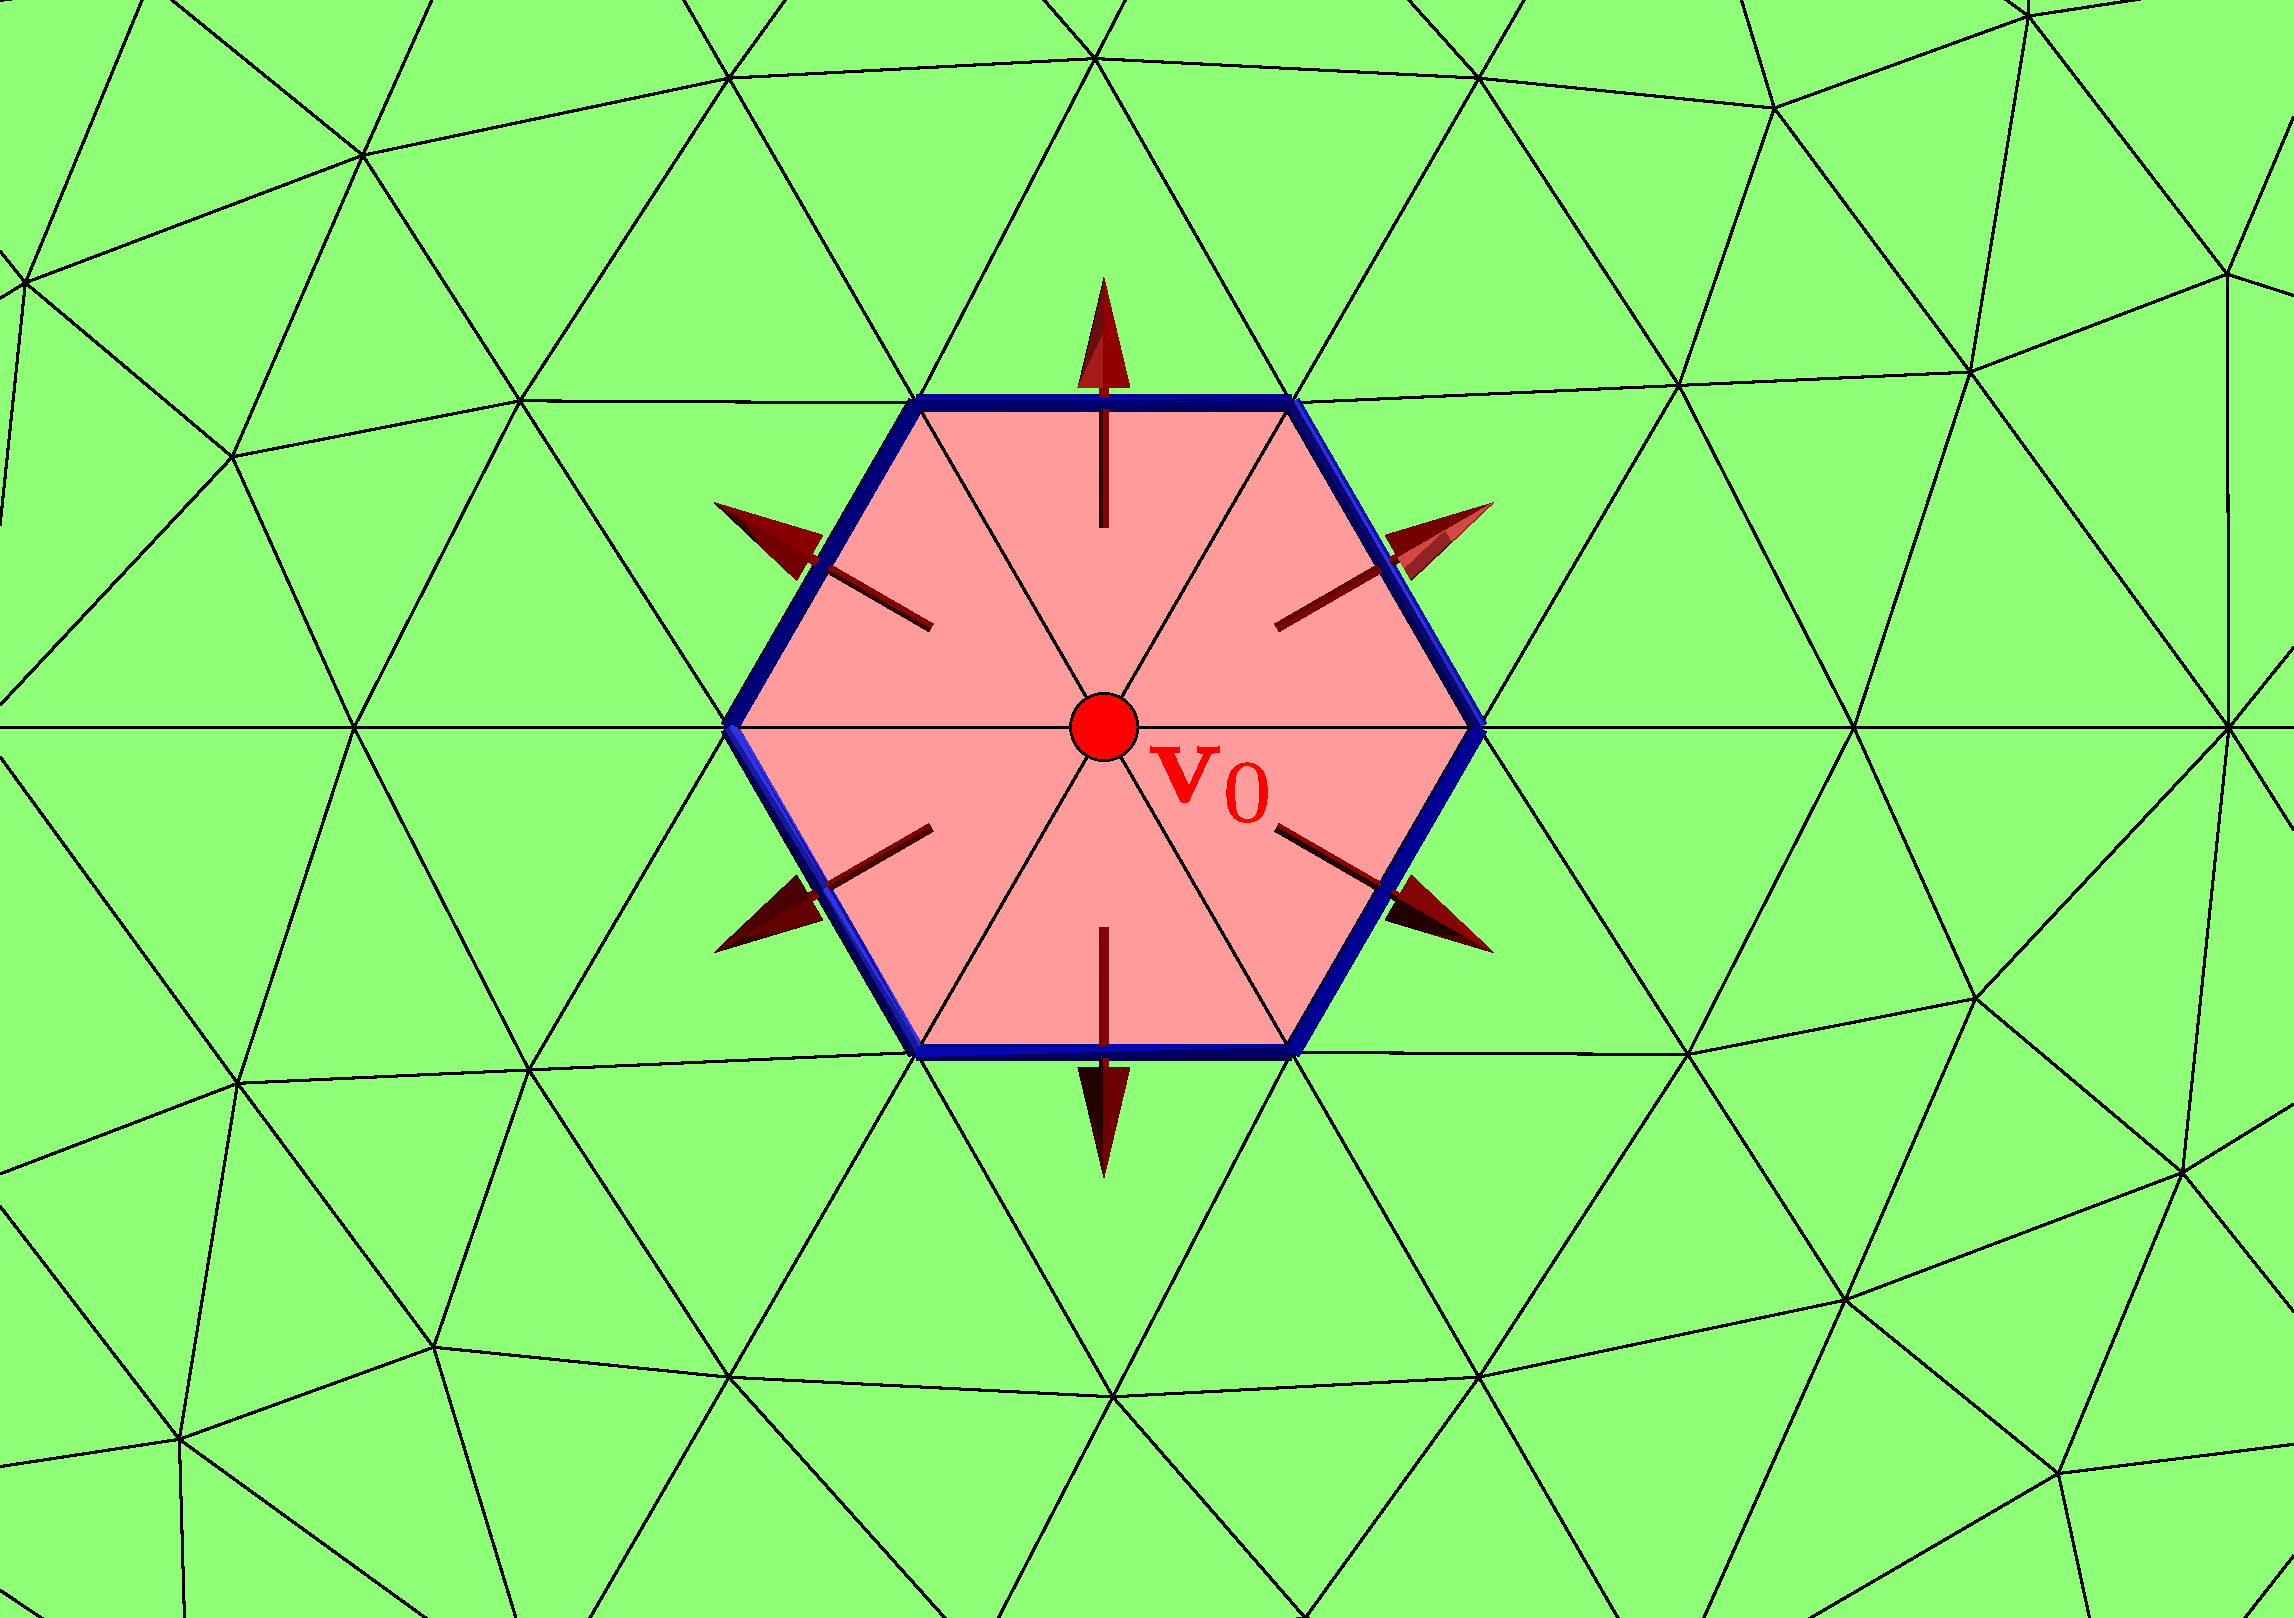
\includegraphics{PointPort.pdf}} \\
\textbf{(a)}\\
\resizebox{0.5\textwidth}{!}{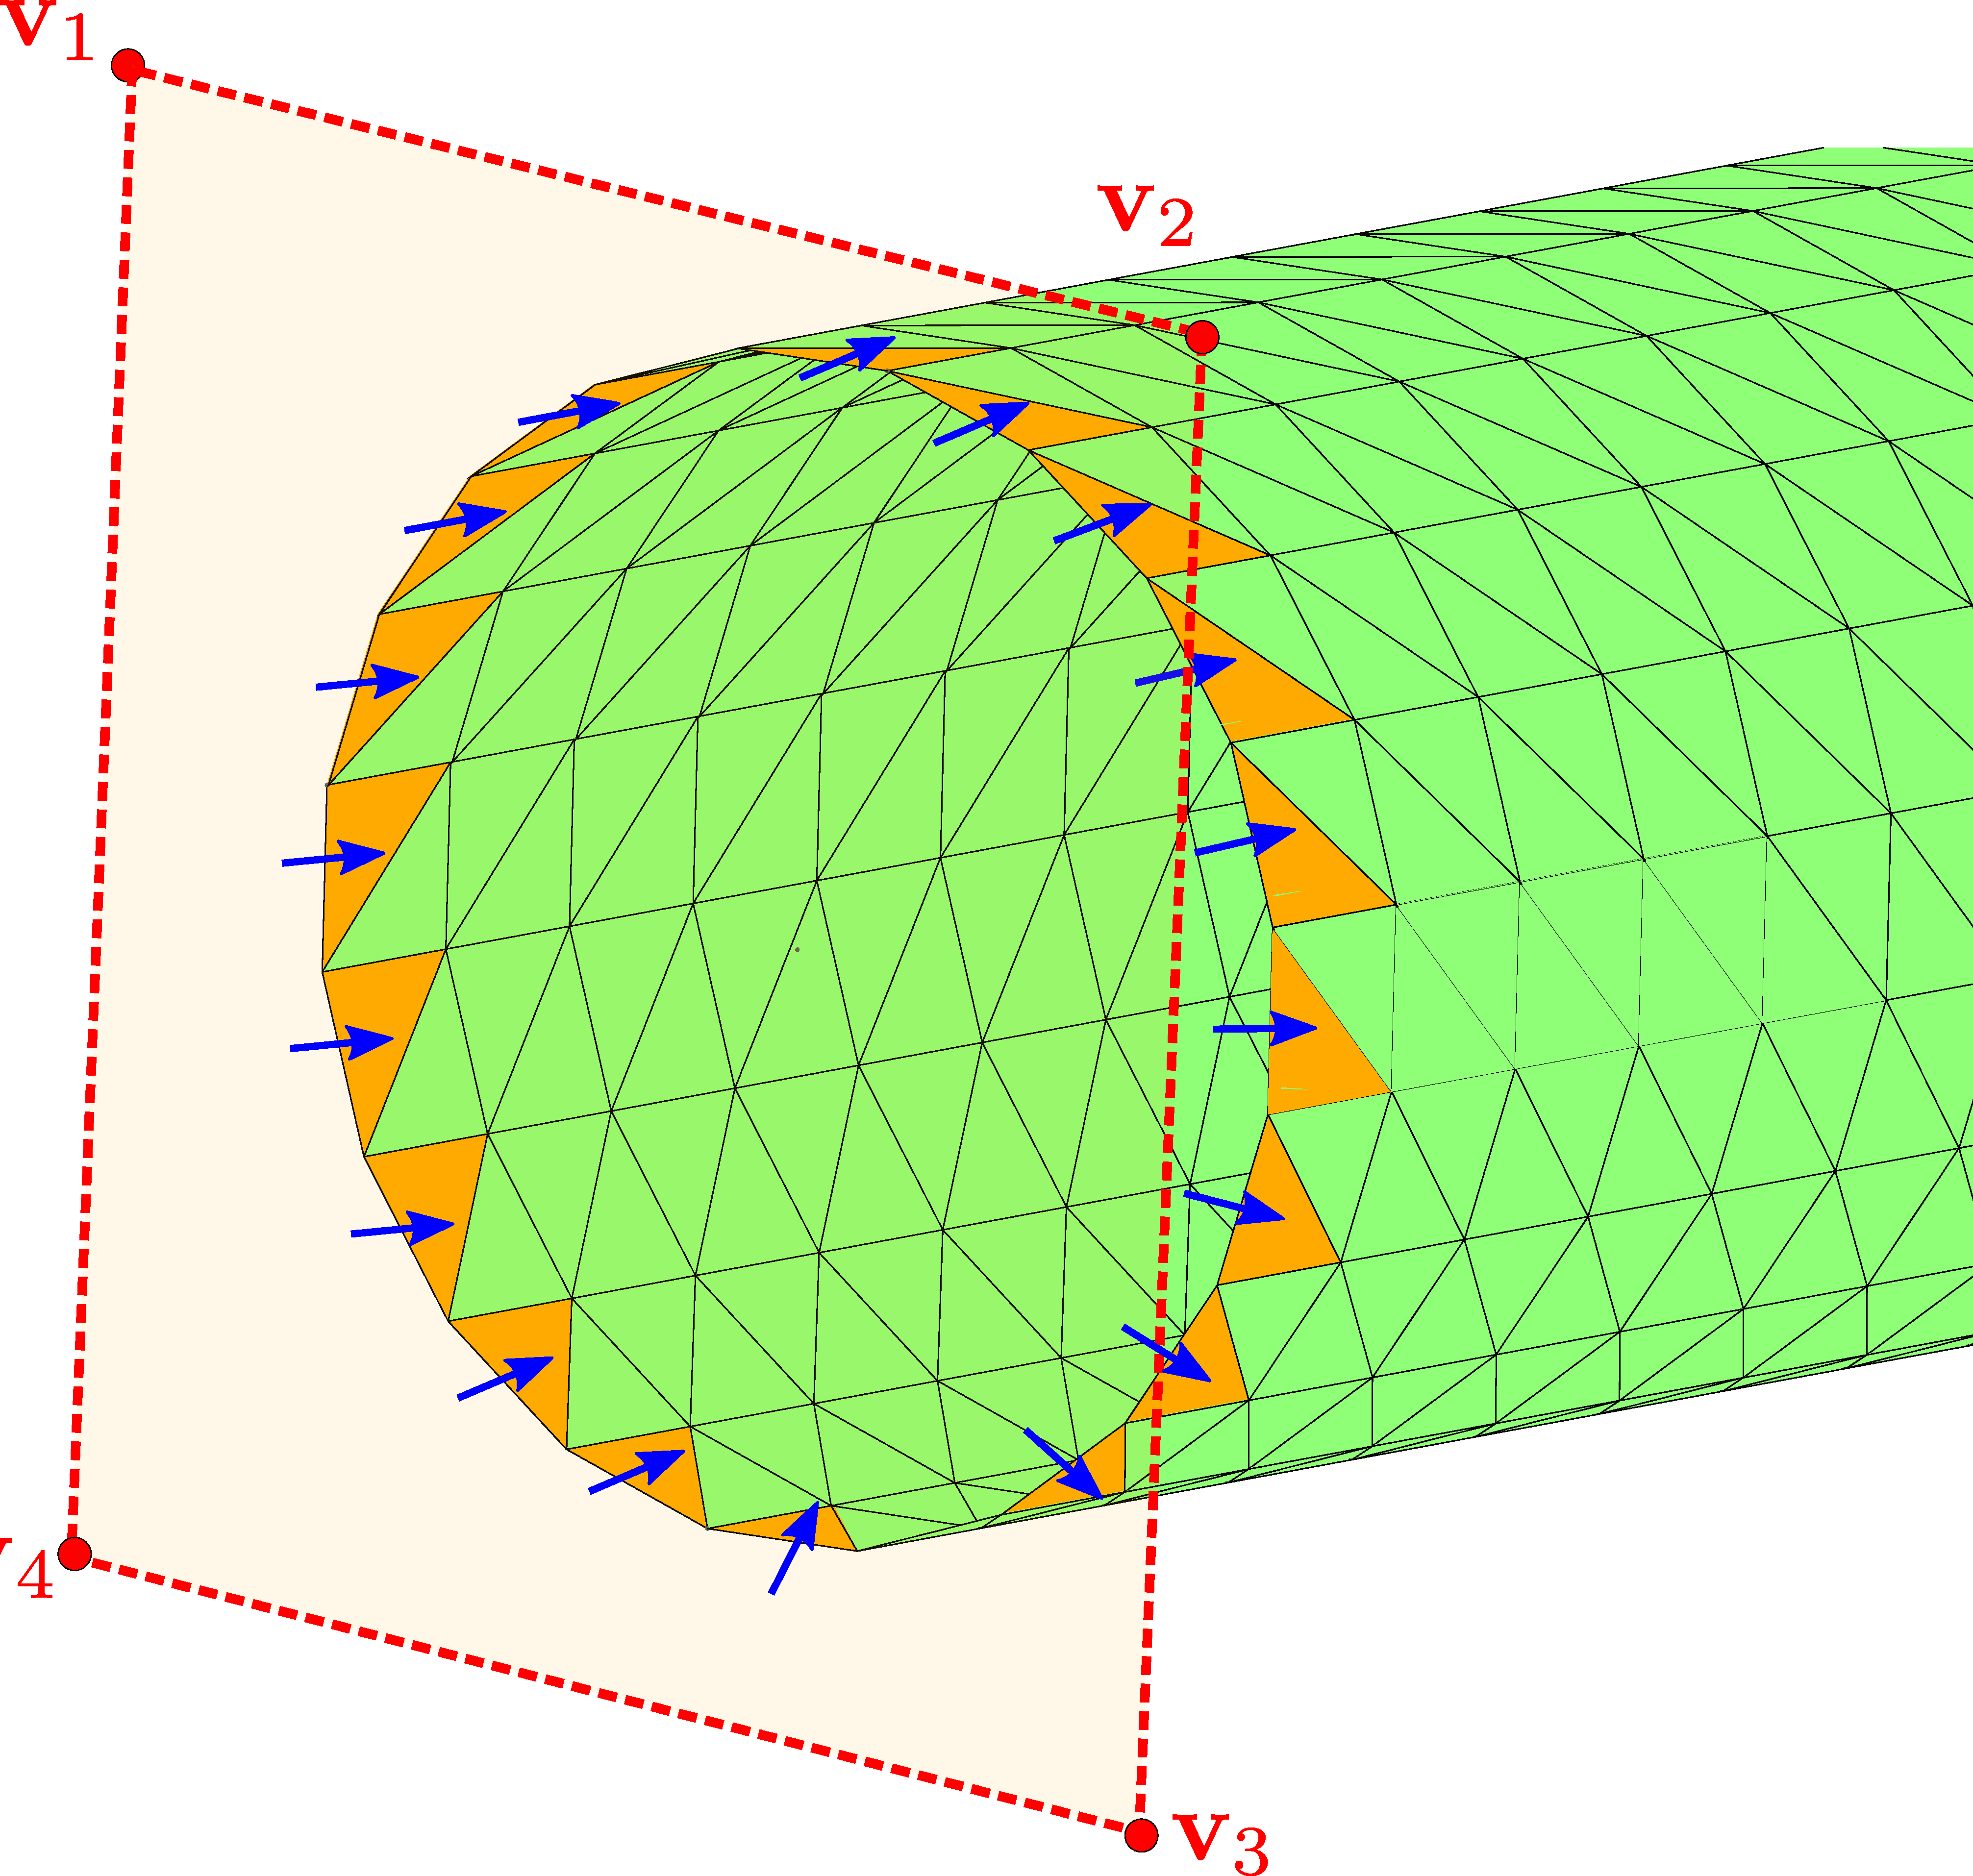
\includegraphics{PolygonPort.pdf}} \\
\textbf{(b)}
\end{tabular}
\begin{tabular}{c}
\resizebox{0.5\textwidth}{!}{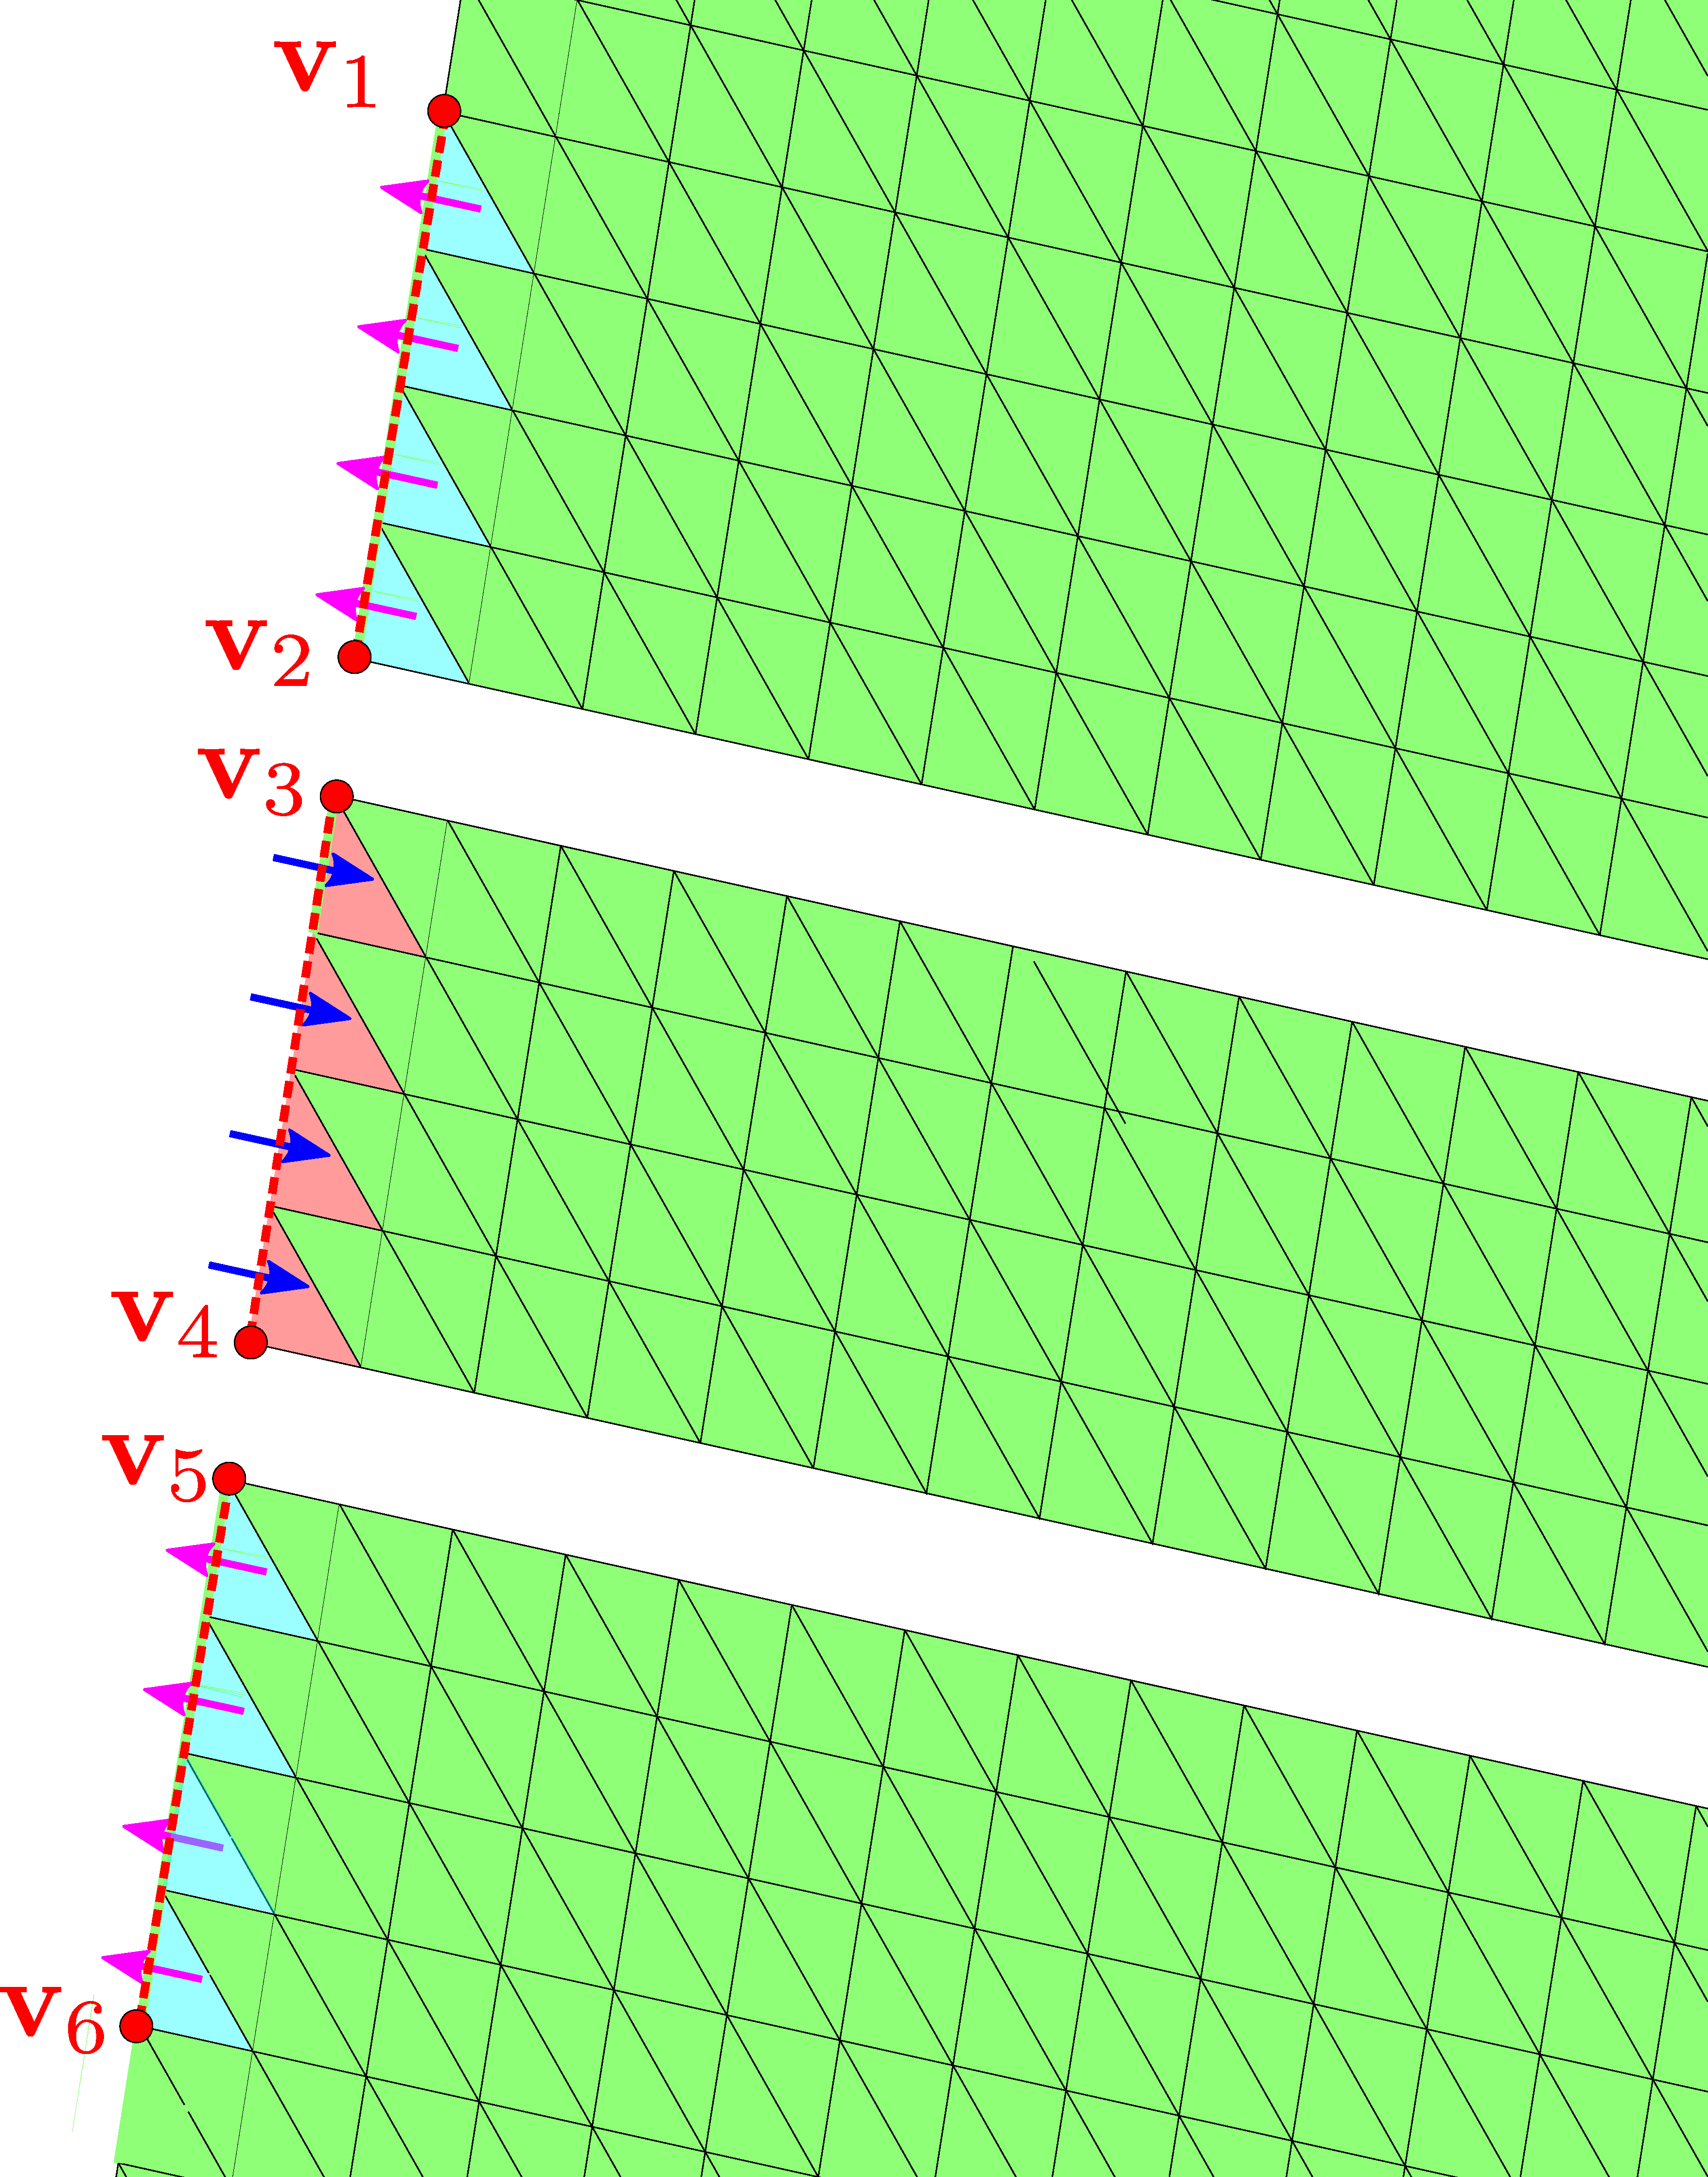
\includegraphics{LinePort.pdf}}\\
\textbf{(c)}
\end{tabular}
\end{tabular}
\caption{Examples of \texttt{RWGPort} terminals.
         \textbf{(a)} Port terminal defined by a single point $\vb v_0$ in the
         interior of a meshed surface. 
         \textbf{(b)} Port terminal defined by a planar polygon; the port terminal
          is the union of all triangle edges lying on the boundary of 
          the meshed structure and inside the polygon.
         \textbf{(c)} Port terminals defined by line segments: the
         positive port terminal (blue arrows) consists of all triangle edges
         on the boundary of the meshed structure lying within the line segment 
         $\overline{\vb v_3 \vb v_4}$, while the negative terminal (red arrows)
         consists of all triangle edges contained in line segments
         $\overline{\vb v_1 \vb v_2}$ and $\overline{\vb v_5 \vb v_6}.$
        }
\label{RWGPortFigure}
\end{center}
\end{figure}
%####################################################################%
%####################################################################%
%####################################################################%

The key extension of the \lss core library provided by {\sc scuff-rf}
is the idea of an \texttt{RWGPort}. This is a physical region of
a material body that interfaces with RF circuitry. More specifically,
a port consists of a positive terminal and an (optional) negative terminal, 
where each terminal is a small region of a surface into (or from)
which an external current is forced; if the port current is $I$, 
then a total current $I$ is forced into the positive terminal
and an equal current is extracted from the negative terminal.
The fields radiated by the resulting
spatially localized current distributions then constitute the incident
field in a scattering problem.
(A port may have no negative terminal, in which case the current
forced into the positive terminal may be thought of as flowing out 
through the ground plane of the substrate (if present) or from 
a negative terminal at spatial infinity.

Figure \ref{RWGPortFigure} shows some examples of \texttt{RWGPort}
terminals. As this figure makes clear, each port is fully defined
by one or more vertices; ports are specified to {\sc scuff-em}
simply by giving the coordinates of these vertices.

To each \texttt{RWGPort} terminal correspond one or more triangles with distinguished
edges (indicated by arrows in Figure \ref{RWGPortFigure}), to which {\sc scuff-em}
assigns \textit{half-RWG} basis functions $\vb h(\vb x)$.
A half-RWG basis function is just what it sounds like---it is defined by
a single triangle, with a distinguished choice of vertex, and it describes
a surface-current density supported only on that triangle,
emanating from the vertex and flowing normally outward through the opposite edge.
In a \textit{full}-RWG function $\vb b(\vb x)$ this outflow of current is
sunk into the adjacent panel (which, in {\sc scuff-em} parlance, would be
the `negative panel' of the full RWG function), and thus full RWG
functions carry no net current; half-RWG functions, on the other hand,
have no negative panel and describe currents that appear from out of nowhere,
as is appropriate for representing ports driven by a given current injected
by fixed external sources.

The \textit{perimeter} of a port terminal is the sum of the lengths of
all triangle edges it contains. This number is relevant for determining
the weight with which each half-RWG basis function in a port terminal is
populated to describe a port current $I$.
If $L_{p}^\pm$ are the perimeters of the positive and negative ports
of port $p$, then a port current $I_p$ is described by weighting
each basis function in the positive terminal with weight
$+\frac{I_p}{L_p^+}$ and 
each basis function in the negative terminal with weight
$-\frac{I_p}{L_p^-}$. 
Thus, defining
%%%%%%%%%%%%%%%%%%%%%%%%%%%%%%%%%%%%%%%%%%%%%%%%%%%%%%%%%%%%%%%%%%%%%%
\begin{align}
\vb K_p(I_p; \vb x)
&\equiv \left(\parbox{0.6\textwidth}
    { spatial distribution of electric surface-current density
      due to port $p$ driven by current $I_p$
    }
  \right)
\intertext{we have}
\vb K_p(I_p; \vb x)
&= \frac{I_p}{L_p^+} \sum_{a\in \mc{P}_p^+} \vb h_{a}(\vb x)
  -\frac{I_p}{L_p^-} \sum_{a\in \mc{P}_p^-} \vb h_{a}(\vb x).
\label{KpDef}
\end{align}
%%%%%%%%%%%%%%%%%%%%%%%%%%%%%%%%%%%%%%%%%%%%%%%%%%%%%%%%%%%%%%%%%%%%%%
where the notation $a\in \mc P_p^\pm$ indicates that
$a$ runs over the indices of all half-RWG basis functions
on the $\pm$ terminal of port $p$. 

In this memo I use indices $a,b$ for half-RWG functions 
and $\alpha,\beta$ for full-RWG functions.

\paragraph{Some technical implementation details} 
Any meshed representation of an open surface in a {\sc scuff-em} geometry 
is automatically assigned a set of half-RWG basis functions, one 
for each exterior panel edge; these are stored 
within the \texttt{RWGSurface} structure for the surface
in an array called \texttt{HalfRWGEdges}. 
(Full RWG edges are stored separately, in the \texttt{Edges} array.)
Ordinarily, the half-RWG functions assigned to exterior edges are inert
in {\sc scuff-em} scattering problems; they are identified when the 
geometry is read and their properties are stored in the \texttt{HalfRWGEdges} 
array, but they are never populated with surface-current weights 
and do not contribute to the SIE system or to post-processing quantities. 
However, when a half-RWG function for an exterior edge is identified as 
belonging to a port terminal, it is promoted to an active participant 
in scattering calculations, contributing to the RHS vector and to 
post-processing quantities like scattered fields.

In addition to ports defined on boundaries of open surfaces, it is
also possible to define ports based at individual vertices
in the \textit{interior} of surfaces. In this case, although the panels
that share that vertex already belong to full-RWG functions,
we create separate new half-RWG functions for them to describe 
their their role in supporting the port-current distribution.
Thus, each instantiation of a point-based port results in the 
creation of new \texttt{HalfRWGEdge} structures that are tacked on 
to the end of the \texttt{HalfRWGEdge} array for the \texttt{RWGSurface}
in question.

%%%%%%%%%%%%%%%%%%%%%%%%%%%%%%%%%%%%%%%%%%%%%%%%%%%%%%%%%%%%%%%%%%%%%%
%%%%%%%%%%%%%%%%%%%%%%%%%%%%%%%%%%%%%%%%%%%%%%%%%%%%%%%%%%%%%%%%%%%%%%
%%%%%%%%%%%%%%%%%%%%%%%%%%%%%%%%%%%%%%%%%%%%%%%%%%%%%%%%%%%%%%%%%%%%%%
\newpage

\section{SIE scattering problems with port excitation}
\label{SIEWithPortExcitationSection}

In RF device modeling, structures are excited by user-specified input currents
forced into one or more ports of a structure, and the objective is to compute
impedance parameters (or admittance parameters or $S$-parameters) for the 
multiport network (possibly accompanied by other quantities such as 
radiated-field profiles).

On the other hand, in the usual surface-integral-equation (SIE)
approach to electromagnetic scattering implemented by the {\sc scuff-em}
core library, the excitation is provided by a user-specified
incident electromagnetic field configuration (such as a plane wave
or the field of a point dipole),
and the objective is to compute quantities such as absorbed or scattered
power.

How do we squeeze the former problem into the latter framework?
In essence, we take the incident field in the SIE scattering problem
to be the field radiated by the currents forced into the ports
of a structure, and we obtain impedance-matrix elements by calculating
complex power dissipation in the structure.
In this section I discuss how these steps are implemented
in the {\sc scuff-em} RF module.
(The problem of computing fields radiated by port-driven structures
requires no new implementation beyond the existing {\sc scuff-em} 
algorithms for computing fields radiated by excited structures.)

\subsection{Port currents: A new type of incident field}

Consider an $N$-port RF device geometry driven by a set of 
$N$ complex-valued currents $\{I_p\}, p=1,\cdots,N.$
The full surface-current distribution of all driven ports
is given by superposing (\ref{KpDef}) for all ports:
%====================================================================%
\begin{align*}
 \vb K\sups{port}(\vb x)
&= \sum_{a\in \mc P_p^\pm } 
   \underbrace{\pm \frac{I_p}{L_p^{\pm}}}_{\xi_a} \vb h_{a}(\vb x)
\end{align*}
%====================================================================%
The electric field radiated by this current distribution, which defines
the incident field in the scattering problem solved by {\sc scuff-em},
is then a sum of contributions from HRWG basis functions:
%====================================================================%
\begin{align}
  \vb E\sups{inc}(\vb x)
&=\underbrace{\int \vbGamma(\vb x, \vb x^\prime) \cdot \vb K(\vb x^\prime) \, d\vb x^\prime
             }_{\vbGamma\star \vb K}
\\
&= \sum_{a}\xi_a \vbGamma \star \vb h_a
\label{EInc}
\end{align}
%====================================================================%
with $\vbGamma\equiv \vbGamma\supt{EE}$ the $3\times 3$ dyadic Green's function
giving the electric field of an electric current in the medium
of the scattering geometry.\footnote{In a homogeneous
medium with wavevector $k$ and relative wave impedance $Z_r$ we have
$\vbGamma\supt{EE}(\vb x, \vb x^\prime)=ik Z_0 Z_r \mb G(k; \vb x-\vb x^\prime)$
with 
$\mb G_{ij}(\vb r) \equiv \left(\delta_{ij} + \frac{1}{k^2}\partial_i \partial_j\right)
 \frac{e^{ik|\vb r|}}{4\pi |\vb r|}$ the usual Helmholtz dyadic, 
but this discussion is more general; in particular, $\vbGamma\supt{EE}$ may
include the effect of a layered dielectric substrate.}

The usual EFIE formulation of scattering from PEC bodies then 
yields an integral equation for the unknown electric surface-current 
density $\vb K\sups{ind}$ induced on the scatterers by the incident field:
%====================================================================%
\begin{align}
 \int \vbGamma_{\parallel}(\vb x, \vb x^\prime) \cdot \vb K\sups{ind}(\vb x^\prime) d\vb x^\prime
&=-\vb E_\parallel\supt{inc}(\vb x)
\intertext{Inserting (\ref{EInc}),
           expanding $\vb K\sups{ind}$ as a linear combination of RWG basis functions
           $\vb K\sups{ind}=\sum k_\alpha \vb b_\alpha$, and Galerkin testing yields
           a discrete linear system for the expansion coefficients:}
\vb M \cdot \vb k &= \vb r
\label{Mkr}
\end{align}
%====================================================================%
where the elements of $\vb M$ are the $\vbGamma$ interactions of
full RWG basis functions,
%====================================================================%
$$ \vb M_{\alpha\beta} = \Vmv{\vb b_{\alpha}}{\vbGamma}{\vb b_\beta} $$
%====================================================================%
and the elements of the RHS vector are $\vbGamma$ interactions 
of full RWG functions with half RWG functions:
%====================================================================%
\numeq{rAlphaDef}
{r_{\alpha} = -\sum_{a} \xi_a \Vmv{\vb b_{\alpha}}{\vbGamma}{\vb h_a}.}
%====================================================================%
where the sum runs over all edges on all port terminals
and $\xi_a\equiv \pm \frac{I_p}{L_p^\pm}$ is the common
weight of all half-RWG functions $\vb h_a$ on the $\pm$ terminal
of port $p$.
Formally solving (\ref{Mkr}), the induced surface-current density reads
%====================================================================%
\begin{align} 
 \vb K\sups{ind}(\vb x)
&= \sum_{\alpha} k_\alpha \vb b_\alpha(\vb x)
\nn
&= \sum_{\alpha\beta} \vb b_\alpha(\vb x) W_{\alpha\beta} r_\beta
\label{KInd}
\end{align} 
%====================================================================%
with $\vb W=\vb M^{-1}$ the inverse EFIE matrix.

%####################################################################%
%####################################################################%
%####################################################################%
\begin{figure}
\begin{center}
%\includegraphics{PortCurrentIncidentField}}
\caption{The incident field in the BEM scattering problem
         is the field radiated by half-RWG basis functions
         associated with the exterior edges comprising the
         \texttt{RWGPort}.
         Each half-RWG basis function is populated with
         a strength proportional to the port current.
        }
\label{PortCurrentFigure}
\end{center}
\end{figure}

%####################################################################%
%####################################################################%
%####################################################################%
\newpage
\section{Calculation of impedance matrix}

For an $N\subt{P}$-port system driven by a set of port currents $\{I_p\}$,
the complex power is a quadratic function of the $\{I_p\}$,
whose coefficients define the \textit{impedance parameters} $Z_{pq}$
(entries of the \textit{impedance matrix} $\vb Z$) of the system:
%====================================================================%
\numeq{ZpqDef}
{ \frac{1}{2} \int \vb K^* \cdot \vb E \, dA
   \equiv \frac{1}{2}\sum I^*_p Z_{pq} I_q
   = \frac{1}{2} \vb I^\dagger \vb Z \vb I
}
%====================================================================%
where the integral extends over all surfaces in the SIE geometry.
(Note that we consider the full \textit{complex} power, i.e. both
real and imaginary parts of the integral of $\vb J^*\cdot \vb E$.)

In this section I derive an expression relating the impedance parameters $Z_{pq}$
to quantities computed by {\sc scuff-em}. The derivation proceeds in 
multiple steps.

\begin{description}

\item[1. Total surface current.]

For a $N\subt{P}$-port system driven by port currents $\{I_p\}$,
the total surface current at a point $\vb x$ on a meshed surface
is a linear function of the $\{I_p\}$:
%====================================================================%
\begin{align*}
\vb K(\vb x) &= \sum I_p \vb K_p(\vb x)
\\
\end{align*}
%====================================================================%
where $\vb K_p$ receives both a \textit{direct} contribution from the
half-RWG basis functions $\{\vb h(\vb x)\}$ carrying the port currents
and an \textit{induced} contribution from the full-RWG basis
functions populated by the coefficients obtained by solving
the scattering problem, equation (\ref{KInd}):
%====================================================================%
\numeq{Kp}
{\vb K_p(\vb x) =
   \sum_{a\in\mc{P}_p^\pm}
   \pm \frac{1}{L_p^\pm}
   \bigg\{  \vb b_a(\vb x)
           -\sum_{\alpha\beta} \vb b_\alpha(\vb x) W_{\alpha\beta} r_{\beta a}
   \bigg\}
}
%====================================================================%
\item[2. Total electric field.]

The total $\vb E$-field is similarly linear the $\{I_p\}$:
%====================================================================%
\begin{align}
 \vb E(\vb x) 
&= \sum_p I_p \vb E_p(\vb x), 
\quad
\vb E_p(\vb x) 
&= \sum_{b\in\mc{P}^\pm_p}
   \pm \frac{1}{L_p^\pm}
   \bigg\{  \mb E_a(\vb x)
           -\sum_{\alpha\beta} \mb E_\alpha(\vb x) W_{\alpha\beta} r_{\beta a}
   \bigg\}
 \label{Ep}
\end{align}
%====================================================================%
where $\{\mb E_\alpha, \mb E_a\}\equiv \vbGamma \star \{\vb b_\alpha, \vb b_a\}$
are the electric fields due to individual
full- or half-RWG functions weighted with unit strength.
%====================================================================%
\item[3. Complex power.]
Inserting (\ref{Kp}) and (\ref{Ep}) into (\ref{ZpqDef}), the
impedance parameter $Z_{pq}$ becomes a sum of 4 terms:
%====================================================================%
\begin{align*}
 Z_{pq} 
 &\equiv \frac{1}{2}\int \vb J_p(\vb x) \vb E_q(\vb x)\,d\vb x
\\
 &= T_1 + T_2 + T_3 + T_4
\\
\intertext{The first term describes interactions between half-RWG basis functions:}
T_1 &\equiv \sum_{a b} \frac{1}{2 L_p^\pm L_q^\pm} \Inp{\vb h_a}{\vb E_b}
\\
\intertext{The second two terms describe interactions between half-RWG and full-RWG functions:}
T_2 &= -\sum_{a \alpha \beta b}
  \frac{1}{2L_p^\pm L_q^\pm}
 \underbrace{\Inp{\vb b_a}{\vb E_\alpha}}_{r_{p \alpha}}
  W_{\alpha\beta}
  r_{q \beta}
\\
 &= -\frac{1}{2}\vb r^T_p \vb W \vb r_q
\\
T_3 &= -\frac{1}{2}\vb r^T_q \vb W \vb r_p
\\
\intertext{The final term describes the interaction of full-RWG and full-RWG functions:}
 T_4 &\equiv \sum_{a \alpha\beta\gamma\delta b}
  \frac{1}{2L_p^\pm L_q^\pm}
  r_{p \beta}
  W_{\alpha\beta}
 \underbrace{\Inp{\vb b_\alpha}{\vb E_\gamma}}_{W_{\alpha\gamma}^{-1}}
  W_{\gamma\delta}
  r_{q \delta}
\\
&= + \frac{1}{2L_p^\pm L_q^\pm} \vb r_p^T \vb W \vb r_q
\end{align*}
%====================================================================%
Thus, when the dust settles we find that $|T_2|=|T_3|=|T_4|$
and the impedance parameter reads
%====================================================================%
$$ Z_{pq} = \sum_{\pm} \frac{1}{2L_p^\pm L_q^\pm}
 \Big[ -\vb r^T_p \vb W \vb r_q + \sum_{ab} \Inp{\vb h_a}{\vb E_b} \Big]
$$
\end{description}

\end{document}
